\documentclass[11pt,a4paper]{article}

\usepackage[utf8]{inputenc}
\usepackage[english]{babel}
\usepackage[T1]{fontenc}
\usepackage{lmodern}
\usepackage[hidelinks]{hyperref}
\usepackage{subcaption}
\usepackage{graphicx}

\usepackage{amsmath,amssymb,amsfonts}

\title{}
\author{Malte Stær Nissen}

\begin{document}
\maketitle

Image url: http://cdn.logicspot.com/wp-content/uploads/2011/11/Online-Competitor-Analysis.jpg
\url{http://www.korthalsaltes.com/photo/cubic_shapes/cubic_shape01.jpg}

Interpolation: http://www.mathworks.se/help/matlab/ref/interp1.html

\section{External force derivatives}
%
We compute the derivatives of the two expressions for computing the external force image $F$. This is related to the external energy term $E_\mathcal{E}$ by $E_\mathcal{E}(C) = \sum_{i=1}^n F(C(i))$.
\begin{itemize}
\item Local maxima of gradient magnitude:
\end{itemize}
%
\begin{align}
F &= - \frac12 \| g_\sigma \star \nabla I \|^2 \\
&= - \frac12 \| \nabla I_{\sigma} \|^2 \\
&= - \frac12 (\nabla I_{\sigma x}^2 + \nabla I_{\sigma y}^2)
\end{align}
%
We use the chain rule:
%
\begin{align}
F_x &= - (\nabla I_{\sigma x} \nabla I_{\sigma xx} + \nabla I_{\sigma y} \nabla I_{\sigma xy}) \\
F_y &= - (\nabla I_{\sigma x} \nabla I_{\sigma xy} + \nabla I_{\sigma y} \nabla I_{\sigma yy})
\end{align}
%
\begin{itemize}
\item Zero-crossings of Laplacian of Gaussian:
\end{itemize}
%
\begin{align}
F &= - \frac12 ( g_\sigma \star \Delta I)^2 \\
&= - \frac12 \Delta I_{\sigma}^2 \\
&= - \frac12 (\nabla I_{\sigma xx} + \nabla I_{\sigma yy})^2
\end{align}
%
We use the chain rule:
%
\begin{align}
F_x &= - (\nabla I_{\sigma xx} + \nabla I_{\sigma yy}) (\nabla I_{\sigma xxx} + \nabla I_{\sigma xyy}) \\
F_y &= - (\nabla I_{\sigma xx} + \nabla I_{\sigma yy}) (\nabla I_{\sigma xxy} + \nabla I_{\sigma yyy})
\end{align}
%

\section{Implementation description}

\section{Tests and examples}

\begin{figure}[H]
    \centering
    \begin{subfigure}[t]{0.48\textwidth}
        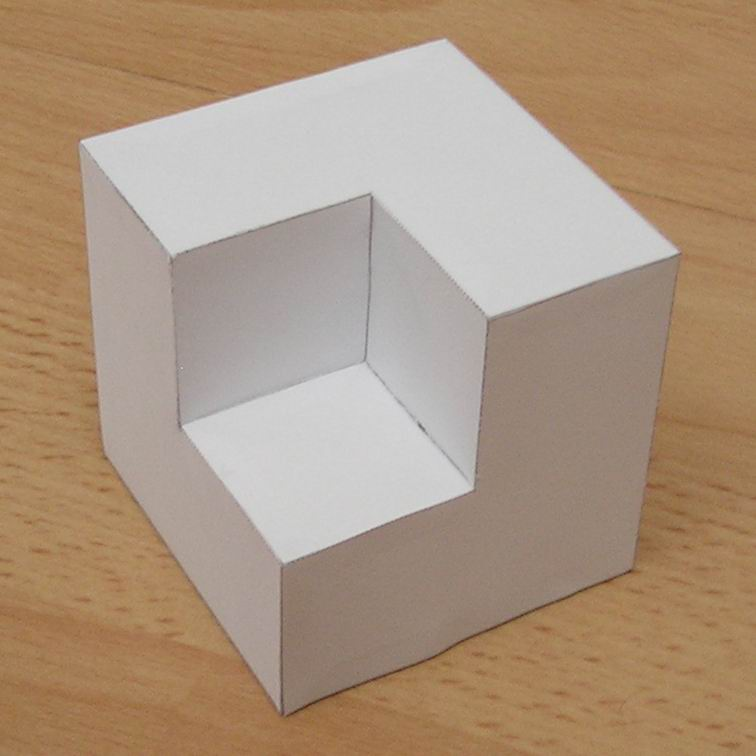
\includegraphics[width=\textwidth]{src/images/cubic_shape01.jpg}
        \caption{original image}
        \label{fig:cubic_original}
    \end{subfigure}
    \begin{subfigure}[t]{0.48\textwidth}
        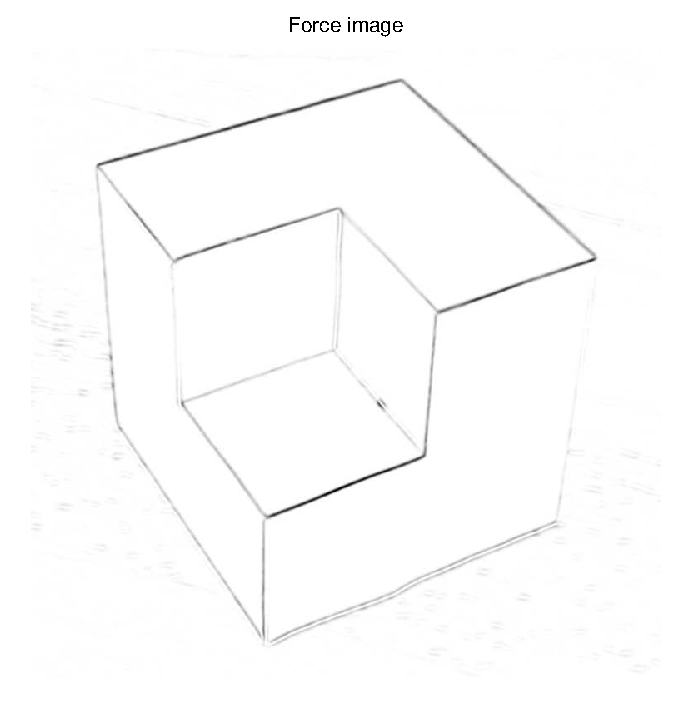
\includegraphics[width=\textwidth]{src/images/cubic_forces.pdf}
        \caption{Force image}
        \label{fig:cubic_forces}
    \end{subfigure}
    \begin{subfigure}[t]{0.48\textwidth}
        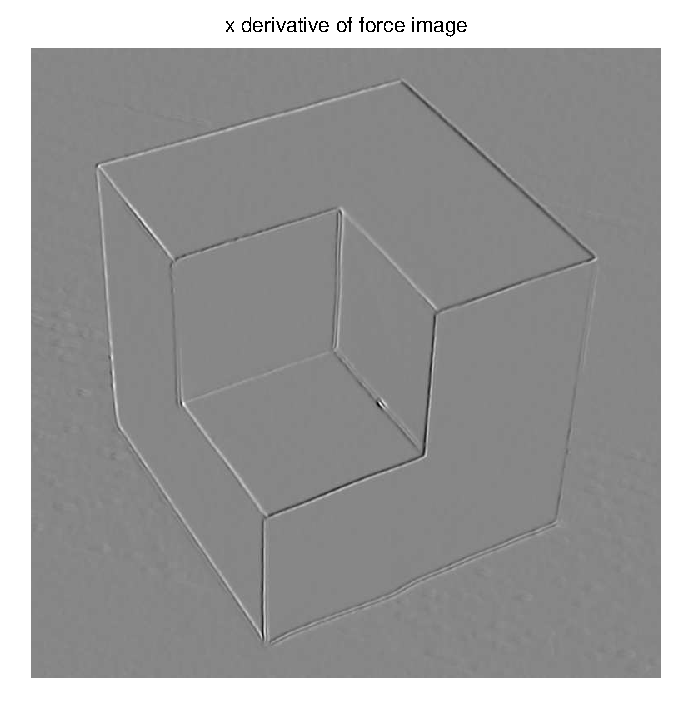
\includegraphics[width=\textwidth]{src/images/cubic_xforces.pdf}
        \caption{x derivative of force image}
        \label{fig:cubic_fx}
    \end{subfigure}
    \begin{subfigure}[t]{0.48\textwidth}
        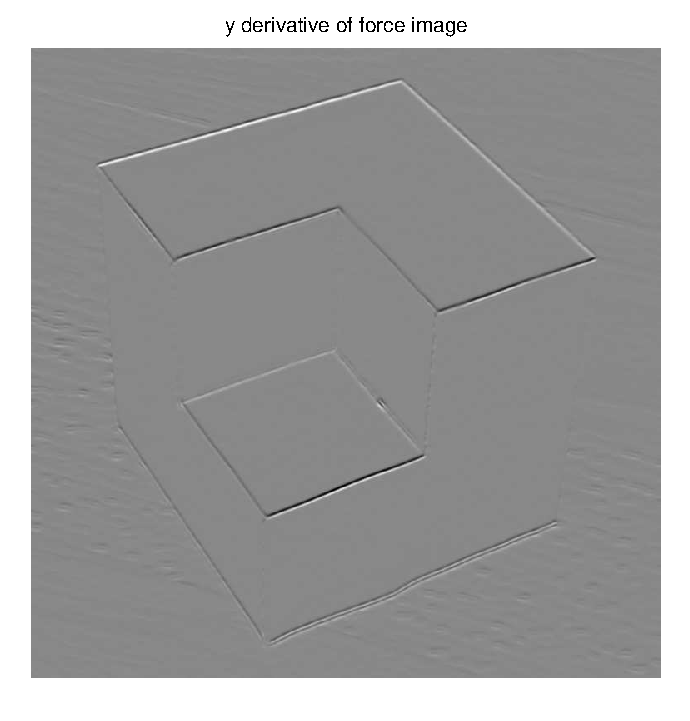
\includegraphics[width=\textwidth]{src/images/cubic_yforces.pdf}
        \caption{y derivative of force image}
        \label{fig:cubic_fy}
    \end{subfigure}
    \caption{\texttt{cubic.jpg} image and snake results}
    \label{fig:cubic}
\end{figure}

\begin{figure}[H]
    \centering
    \begin{subfigure}[t]{0.48\textwidth}
        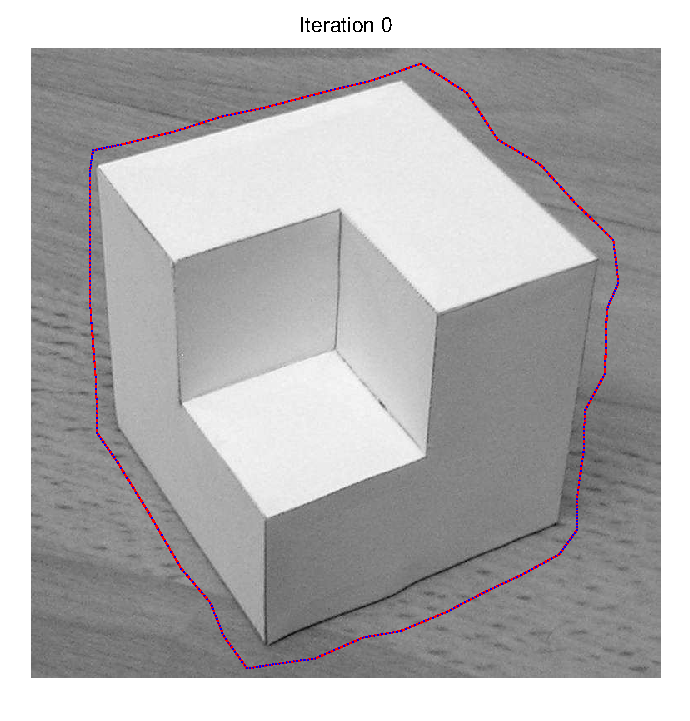
\includegraphics[width=\textwidth]{src/images/cubic_0.pdf}
        \caption{Start}
        \label{fig:cubic_grayscale}
    \end{subfigure}
    \begin{subfigure}[t]{0.48\textwidth}
        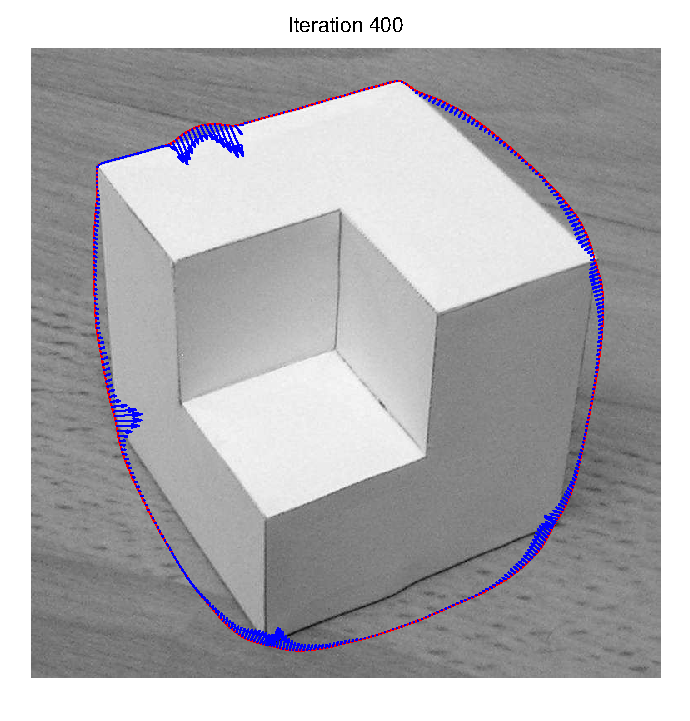
\includegraphics[width=\textwidth]{src/images/cubic_400.pdf}
        \caption{400}
        \label{fig:cubic_400}
    \end{subfigure}
    \begin{subfigure}[t]{0.48\textwidth}
        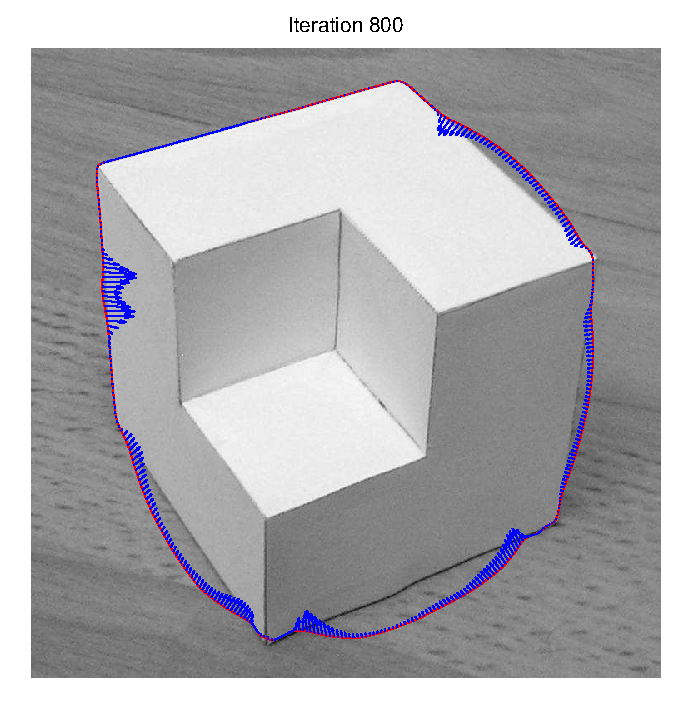
\includegraphics[width=\textwidth]{src/images/cubic_800.pdf}
        \caption{800}
        \label{fig:cubic_800}
    \end{subfigure}
    \begin{subfigure}[t]{0.48\textwidth}
        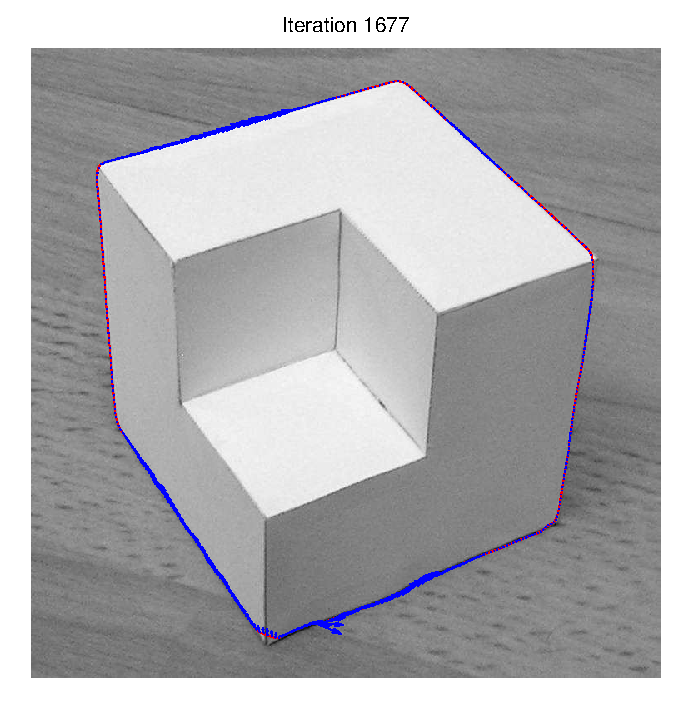
\includegraphics[width=\textwidth]{src/images/cubic_1677.pdf}
        \caption{1677 (end)}
        \label{fig:cubic_end}
    \end{subfigure}
    \caption{\texttt{cubic.jpg} snake intermediate results}
    \label{fig:cubic_intermediate}
\end{figure}

\end{document}

